\documentclass{UoSclass} % Use the Thesis Style

% include your .bib files here
\addbibresource{example_refs.bib}

\begin{document}

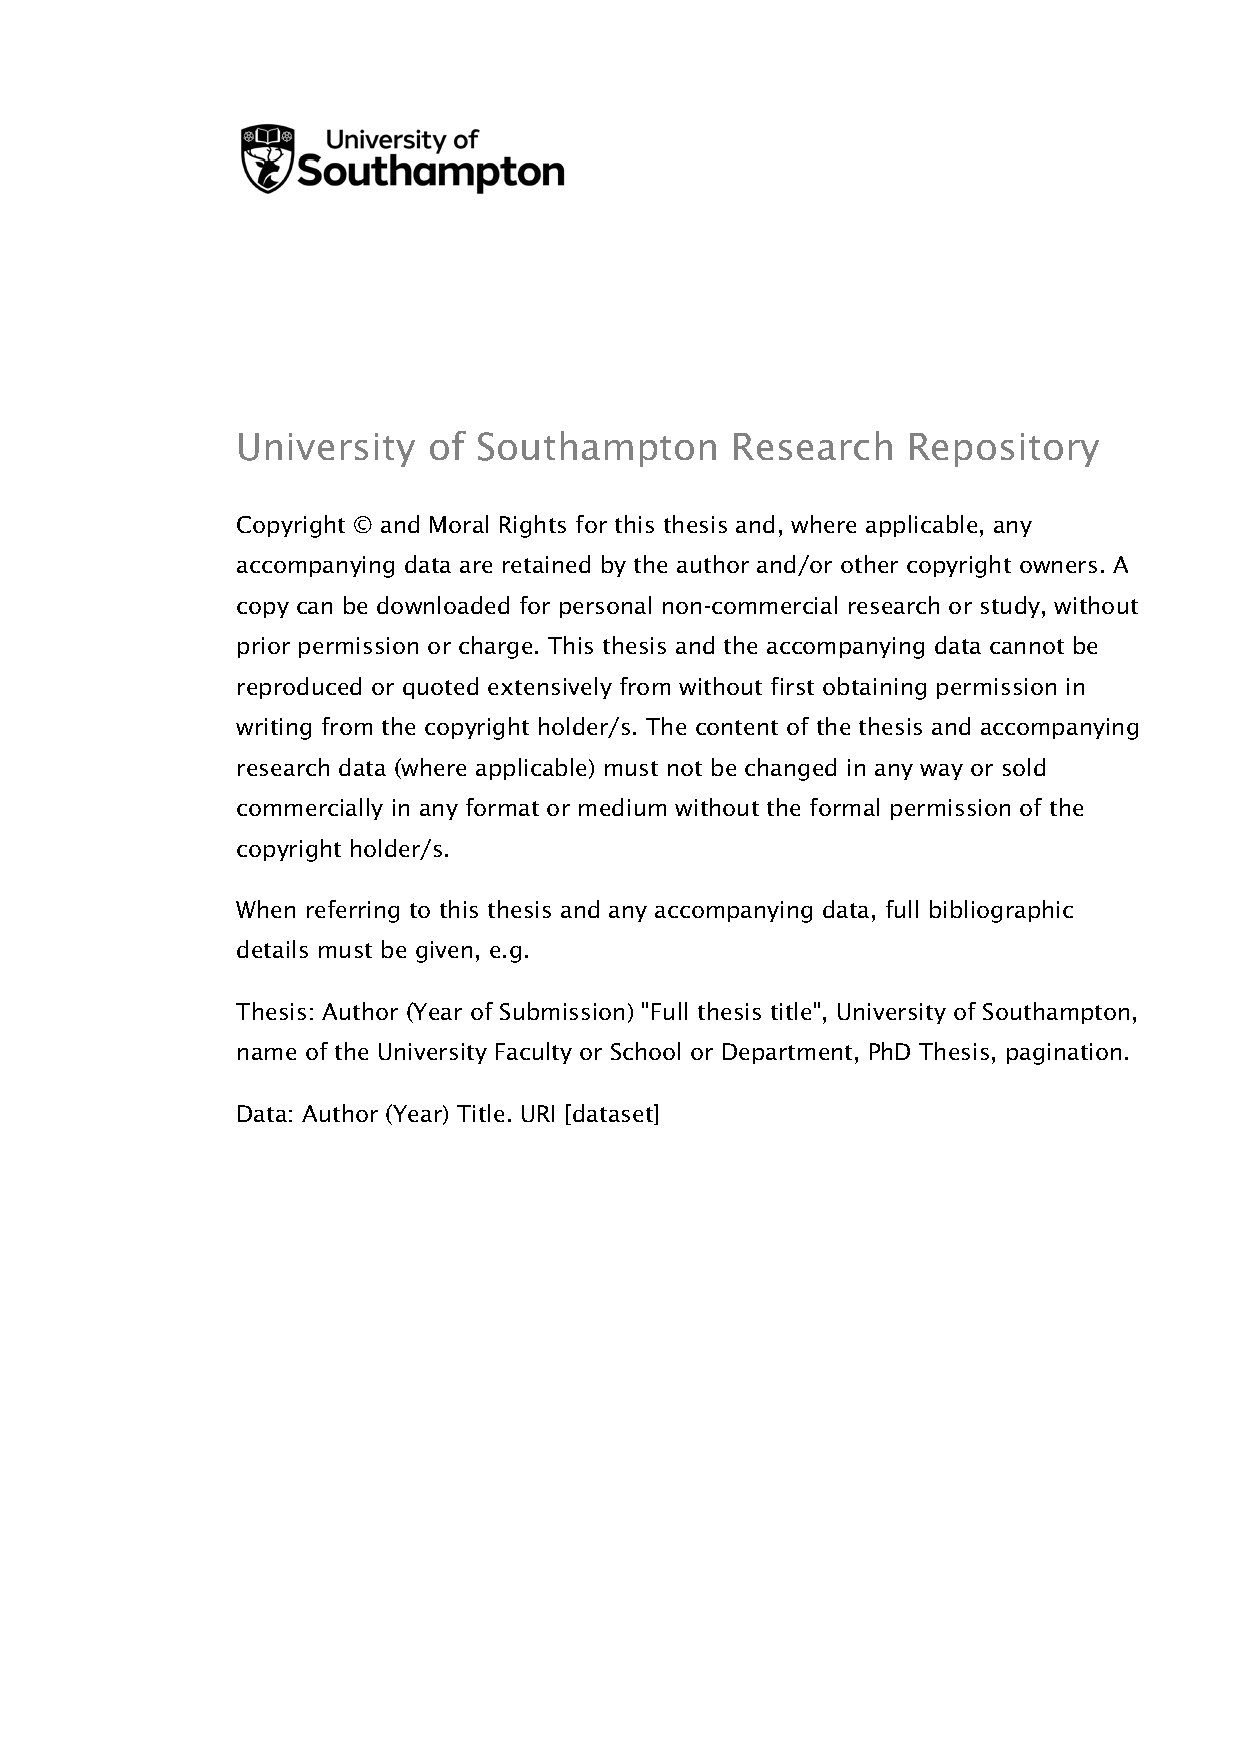
\includepdf[pages={1}]{Thesis_Copyright_Declaration.pdf}
\cleardoublepage
\microtypesetup{protrusion=false}

\begin{titlepage}
    \begin{center}
      
        \centering
        
\includegraphics[width=.4\textwidth]{./figures/UoSlogo2022.eps}         
        
        \vspace{0.5cm}

        \Large
        Faculty\\
        Group\\
        University of Southampton\\
                  
        \vfill

        \Huge
        \textbf{Title}
        
        \vfill

        \LARGE
        \textit{by}  \\
        \textbf{Name}\\
        \Large
        ORCiD:~\href{https://orcid.org/}{ID here}
            
        \vfill

        \textit{A thesis for the degree of\\Doctor of Philosophy}
                  
        \vfill
        \DTMlangsetup{showdayofmonth=false}
        \today
        \vfill
        
      \end{center}
  \afterpage{\blankpage}

\end{titlepage}
\restoregeometry
\thispagestyle{empty}

 \begin{center}
     \textbf{\textcolor{sotonMarineBlue}{University of Southampton}} \\
     \vspace{8pt}
     \underline{Abstract} \\
     \vspace{8pt}
     Faculty \\
     Group \\
     \vspace{8pt}
     \underline{Doctor of Philosophy} \\
     \vspace{8pt}
     \textbf{Title} \\
     \vspace{8pt}
     \textit{by} Name
 \end{center}

\vspace{0.5cm}
\singlespacing

\lipsum[1-4]

\onehalfspacing


\onehalfspacing%set line spacing to 1.5

\pagenumbering{roman}
\pagestyle{plain}
{
  \hypersetup{hidelinks}
  \tableofcontents
  \listoffigures
  \addcontentsline{toc}{chapter}{List of Figures}
  \begingroup
  \clearpage
  \listoftables
  \addcontentsline{toc}{chapter}{List of Tables}
  \endgroup
  \cleardoublepage
}

\phantomsection
\addcontentsline{toc}{chapter}{Accompanying material}
\pagestyle{plain}
\chapter*{Accompanying material}

All data supporting this study are openly available from the University of Southampton repository at DOI: .

\noindent This includes the following:

\cleardoublepage

\phantomsection
\addcontentsline{toc}{chapter}{Declaration of Authorship}
\vspace*{\fill}
\begin{center}{\Large\bf Declaration of Authorship \par}\end{center}
\vspace{15pt}

\noindent I declare that this thesis and the work presented in it is my own and has
been generated by me as the result of my own original research.

\noindent I confirm that:

\begin{enumerate}
\item This work was done wholly or mainly while in candidature for a research degree at this University;
\item Where any part of this thesis has previously been submitted for a degree or any other qualification at this University or any other institution, this has been clearly stated;
\item Where I have consulted the published work of others, this is always clearly attributed;
\item Where I have quoted from the work of others, the source is always given. With the exception of such quotations, this thesis is entirely my own work;
\item I have acknowledged all main sources of help;
\item Where the thesis is based on work done by myself jointly with others, I have made clear exactly what was done by others and what I have contributed myself;
\item Parts of this work have been published as: 
\end{enumerate}

\vspace{15.0mm}
\begin{minipage}[t]{0.7\textwidth}
  Signed:..........................................................................
\end{minipage}%
\begin{minipage}[t]{0.3\textwidth}
  Date:..................
\end{minipage}

\vfill

\cleardoublepage

\phantomsection
\addcontentsline{toc}{chapter}{Acknowledgements}
\pagestyle{plain}

\vspace*{\fill}

\begin{center}{\Large\bf Acknowledgements \par}\end{center}
\vspace{15pt}

\lipsum[1-3]

\vspace{\fill}


\cleardoublepage

\phantomsection
\addcontentsline{toc}{chapter}{Definitions and Abbreviations}
\chapter*{Definitions and Abbreviations}

\acuseall
\printacronyms[display=all,heading=section*,include=acronym,name=Acronyms]
\printacronyms[display=all,heading=section*,include=symbol,name=Symbols]

\cleardoublepage




\pagenumbering{arabic}
\pagestyle{fancy}% set headers/footers
\microtypesetup{protrusion=true}

\chapter{Introduction}
\setcounter{page}{1}

\lipsum[1]

\section{Examples}

Bagavathiappan~\textit{et al.}~\cite{Bagavathiappan2013} suggest that this is a great template, but Liu~\textit{et al.}~\cite{Liu2022} aren't so sure. Maybe these equation examples will convince you:
%
\begin{equation} \label{eq:velocitytext}
    v = \left( \frac{d_{\textrm{aligned}} + d_{\textrm{offset}}}{t_{\textrm{aligned}} - t_{\textrm{wedge}}} \right)
    \tagaddtext{[\si{\meter\per\second}]}
\end{equation} 
%
\begin{equation} \label{eq:velocitynum}
    5099.18 = \left( \frac{0.1 + 0.04587}{5.812{\times}10^{-5} - 2.951{\times}10^{-5}} \right)
    \tagaddtext{[\si{\meter\per\second}]}
\end{equation} 
%

\clearpage

\vspace*{\fill}
\begin{figure}[h]
    \centering
    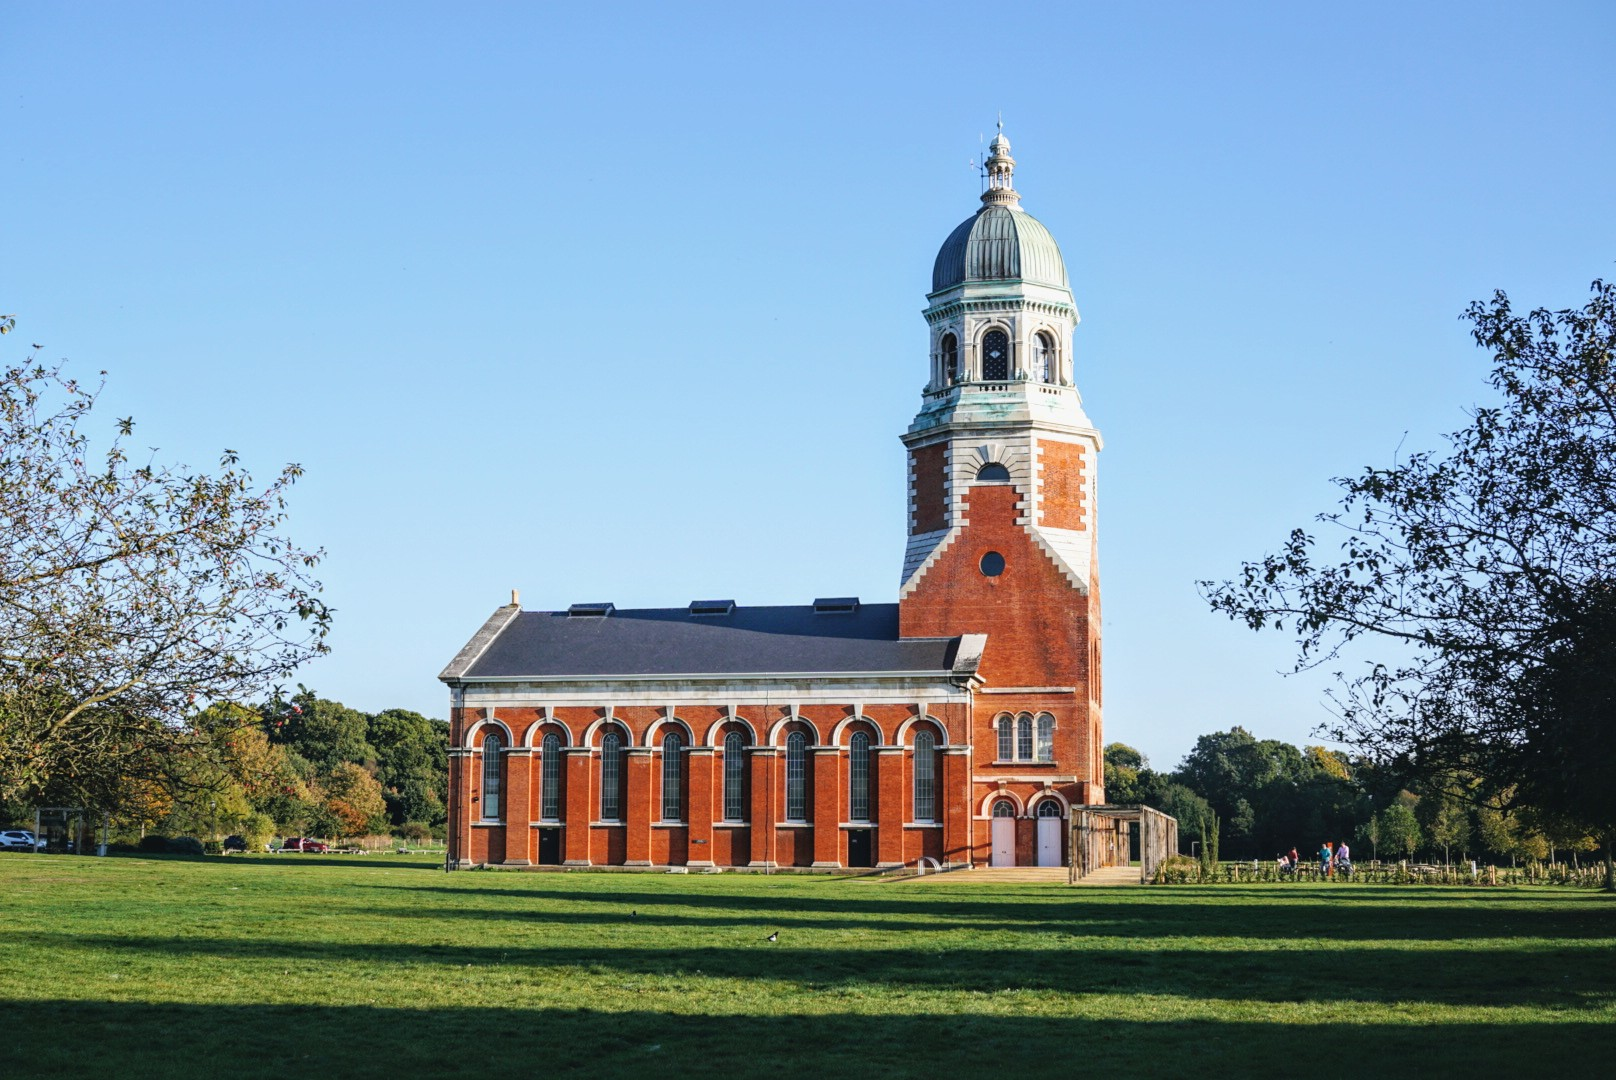
\includegraphics[width=.8\textwidth]{./figures/example_photo.JPG}
    \caption[Royal Victoria Chapel, Southampton]{Royal Victoria Chapel, Southampton.}\label{fig:ngv_photo}
\end{figure}
\vfill
\begin{table}[h]
    \centering
    \begin{tabulary}{\textwidth}{L}
        \toprule
        \textbf{Measurement Hardware}     \\
        \midrule
        2x Olympus ABWX-2001 Variable angle wedges \\
        2x Olympus A539S-SM 1~MHz transducers \\
        Olympus ultrasonic couplant B \\
        GW Instek MFG-2203M Signal generator \\
        Picoscope 3406DMSO USB Oscilloscope \\
        Thermadata T-type temperature loggers \\
        VWR Hot plate \\
        \bottomrule
    \end{tabulary} 
    \caption{Experimental measurement hardware.}\label{table:hardware}
\end{table}
\vfill

% Include chapters here:
% \input{chapter1.tex}

\cleardoublepage
\printbibliography[title={List of references}]
\addcontentsline{toc}{chapter}{List of references}%Including it as a chapter

\end{document}